%!Cau!%
\begin{ex}%[Thử sức trước kì thi đề số 4, THTT, 2019]%[Trần Hòa, 12EX-7-2019]%[1D1G3-7]
	Cho phương trình $2\sin^2x+\sqrt{3}\sin2x-2(\sqrt{3}\sin x+\cos x)-m=0$. Để phương trình chỉ có hai nghiệm $x_1$, $x_2$ thuộc đoạn $\left[-\dfrac{\pi}{3};\dfrac{\pi}{2}\right]$ thì $m\in (a;b)$. Giá trị của $b-a$ là
	\choice
	{$3\sqrt{3}$}
	{$4-2\sqrt{3}$}
	{$4$}
	{\True $4\sqrt{3}-2$}
	\loigiai{
	Đặt $t=\sqrt{3}\sin x+\cos x\quad (*)$\\
	$\Rightarrow t^2=3\sin^2x +\cos^2x+2\sqrt{3}\sin x\cos x =2\sin^2x+\sqrt{3}\sin 2x+1$\\
	$\Rightarrow 2\sin^2x+\sqrt{3}\sin2x=t^2-1$.\\
	Phương trình  đã cho trở thành
	$$t^2-1=2t-m=0\Leftrightarrow m+1=t^2-2t.\quad (1)$$	
	Do $x\in \left[-\dfrac{\pi}{3};\dfrac{\pi}{2}\right]$ nên $t=\sqrt{3}\sin x+\cos x=2\sin\left(x+\dfrac{\pi}{6}\right)\in [-1;2].$
	\immini{Với mỗi $t\in[-1;\sqrt{3})$ thì tương ứng sẽ cho một nghiệm $x$ thuộc đoạn $\left[-\dfrac{\pi}{3};\dfrac{\pi}{2}\right]$ và mỗi $t\in [\sqrt{3};2]$ thì sẽ cho hai nghiệm $x$ thuộc đoạn $\left[-\dfrac{\pi}{3};\dfrac{\pi}{2}\right]$.\\
	Vậy yêu cầu bài toán tương đương với tìm $m$ để phương trình $(1)$ có hai nghiệm phân biệt thuộc $[-1;\sqrt{3})$ hoặc chỉ có một nghiệm thuộc $[\sqrt{3};2]$ và không có nghiệm thuộc $[-1;\sqrt{3})$.}{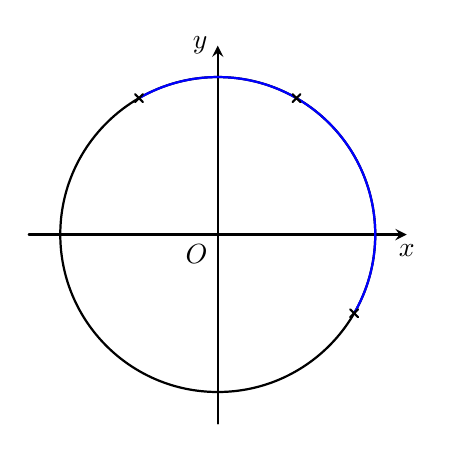
\begin{tikzpicture}[line join=round, line cap=round,>=stealth,thick]
\tikzset{label style/.style={font=\footnotesize}}
\draw[->] (-2.4,0)--(2.4,0) node[below] {$x$};
\draw[->] (0,-2.4)--(0,2.4) node[left] {$y$};
\draw (0,0) node [below left] {$O$};
\draw (0,0) circle (2);
\draw[color=blue,thick] (-30:2cm) arc (-30:120:2);
\foreach \i in {0,3,5}
{
	\draw plot[mark=x] coordinates {({-30+\i*30/1}:2)};
}
\end{tikzpicture}}
Xét hàm số $f(t)=t^2-2t$ có bảng biến thiên

\begin{center}
    \begin{tikzpicture}
\tkzTabInit[nocadre=false,lgt=1.2,espcl=4,deltacl=0.6]
{$t$ /1,$f(t)$ /2.5}{$-1$,$1$,$2$}
%\tkzTabLine{,+,$0$,-,$0$,+,}
\tkzTabVar{+/$3$,-/$-1$,+/$0$}
\tkzTabVal[draw]{2}{3}{0.5}{$\sqrt{3}$}{$3-2\sqrt{3}$}

\end{tikzpicture}

\end{center}
Dựa vào bảng biến thiên ta được 
$$-1<m+1<3-2\sqrt{3}\Leftrightarrow -2<m<2-2\sqrt{3}.$$
Suy ra $a=-2$, $b=2-2\sqrt{3}\Rightarrow b-a=4-2\sqrt{3}.$}	
\end{ex}